Android is mobile operating system developed by Google. It's opensource system based on the Linux kernel mainly used in mobile devices such as smartphones, tablets and smart watches, but it can be found also in devices such as set-top boxes, media players and other electronics.
%Android je mobilní operační systém vyvíjený společností Google, který je založený na Linuxovém jádře. Je vyvíjen jako opensource a používá se především v mobilních zařízeních jako jsou chytré telefony, hodinky a tablety. Můžeme jej však také nalézt také v přístrojích jako jsou set-top boxy, multimediální přehrávače a v jiné elektronice.\\

\section{History}
Android, Inc. was founded in California USA in 2003. Google, Inc. bought Android two years later. In 2007, Google acquired several patents in the field of mobile devices. The same year on November 5, there is official presentation of an association of companies formed the Open Handset Alliance, which aims to create open standards in mobile devices. The first smartphone running Android released on October 22, 2008. Table \ref{androidHistory} presents a brief history of an operating system Android. 
%Počátky Androidu spadají do roku 2003, kdy byla v Kalifornii v USA založena společnost Android, Inc. O Dva roky později firmu odkupuje světoznámá společnost Google. V roce 2007 získává Google několik patentů v oblasti mobilních zařízení a 5. listopadu téhož roku dochází k oficiálnímu představení a vzniká sdružení firem Open Handset Alliance, která mé za cíl vytvoření otevřených standartů v oblasti mobilních zařízení. V tabulce odkaz je zobrazena stručná historie verzí operačního systému Android.

\begin {table}[h!]
    \begin{tabular}{|l|c|l|c|}
    \hline
    {\bf Release date}  & {\bf Version} & {\bf Codename}        & {\bf API level}   \\
    \hline \hline
    September 23, 2008  & 1.0 -- 1.1    & ---                   & 1 -- 2            \\
    \hline
    April 27, 2009      & 1.5           & Cupcake               & 3                 \\
    \hline
    September 15, 2009  & 1.6           & Donut                 & 4                 \\
    \hline
    October 26, 2009    & 2.0 -- 2.1    & Eclair                & 5 -- 7            \\
    \hline
    May 20, 2010        & 2.2 -- 2.2.3  & Froyo                 & 8                 \\
    \hline
    December 6, 2010    & 2.3 -- 2.3.7  & Gingerbread           & 9 -- 10           \\
    \hline
    February 22, 2011   & 3.0 -- 3.2    & Honeycomb             & 11 -- 13          \\
    \hline
    October 18, 2011    & 4.0 -- 4.0.4  & Ice Cream Sandwich    & 14 -- 15          \\
    \hline
    July 9, 2012        & 4.1 -- 4.3    & Jelly Bean            & 16 -- 18          \\
    \hline
    October 31, 2013    & 4.4 -- 4.4.4  & KitKat                & 19 -- 20          \\
    \hline
    November 12, 2014   & 5.0 -- 5.0.2  & Lollipop              & 21                \\
    \hline
    \end{tabular}
    \centering
    \caption{Android version history}
    \label{androidHistory}
\end{table}

\section{Architecture}
Architecture of Android system consists from six layers shown in Figure \ref{androidArchitecture}. We introduce these layers in the following section.
%Architektura systému android je složena z šesti vrstev:

\begin{figure}[h!]
    \centering
    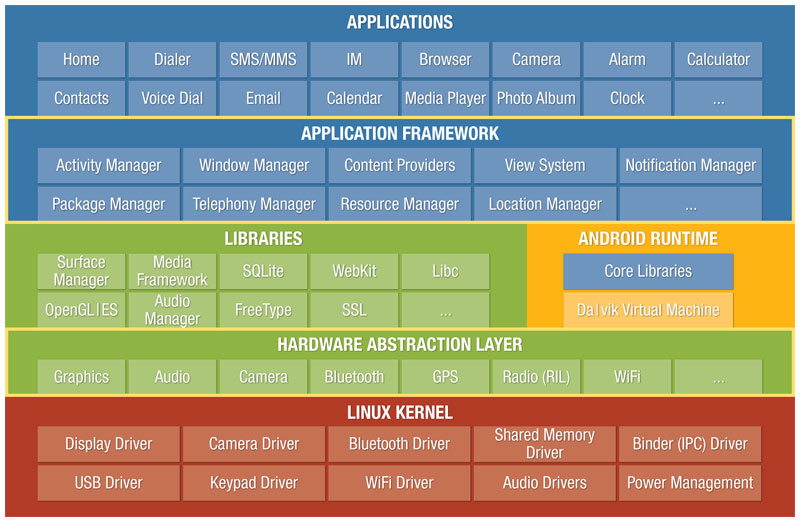
\includegraphics[scale=0.5]{fig/android_architecture.jpg}
    \caption{Android architecture \cite{AndroidArch}}
    \label{androidArchitecture}
\end{figure}

\subsection{Linux kernel} %https://source.android.com/devices/
The lowest layer stands between hardware devices and other architectural layers. Android is based on special version of Linux kernel and several accessories such as memory management system, the Binder IPC driver and others. Since the beginning, Android was built on the Linux 2.6 kernel, the latest Android version runs on the kernel 3.4.
%Tato nejnižší vrstva je postavena mezi hardware zařízení a ostatní vrstvy architektury. Android je postavený na zvlaštní verzi Linuxového jádra a několika speciálními doplňky jako jsou správa systémové paměti, the Binder IPC driver, and other. Od počátku byl android postaven na linuxovém jádru 2.6, nejnověší android pak běží na jádru 3.4.  Při startu se jádro zavede do operační paměti a je mu předáno řízení.

\subsection{Hardware abstraction layer (HAL)} %https://source.android.com/devices/
Hardware abstraction layer is standart interface, which allows android system calls to drivers layer, while he does not care what is the implementation of in the lower layers drivers and hardware. For each piece of hardware should be a driver and matching HAL providing hardware options.
%HAL je standartní rozhraní které umožňuje systému android volat do vrstvy ovladačů, zatímco je mu jedno jaká je implementace v nižších vrstvách obladačů a hardwareru. Pro každý kus hardwaru by měl existovat ovladač a k němu odpovídající HAL poskytující možnosti hardwaru.

\subsection{Libraries}
Above the HAL is a layer of native libraries. These libraries are written in C or C ++. These libraries can be accessed through android sdk, but if direct access is required, it is possible to do this through the Native Development Kit (NDK). These libraries include:
%Nad HAL vrstvu se nachází vrstva nativních knihoven. Tyto knihovny jsou napsány v jazyce C nebo C++. K těmto knihonám se dá přistoupit přes android sdk pokud je však požadován přímý přístup je možné to provést přes NDK. Mezi tyto knihovny patří:

\begin{itemize} %http://www.android-app-market.com/android-architecture.html
\item Surface manager -- library for composing windows on the screen
%knihovna pro skládání oken na obrazovce
\item Media Framework -- provides various multimedia codecs for playing and recording video in various formats
%poskytuje různé multimediální kodeky pro nahrávání a přehrávání videa v různých formátech.
\item SQLite -- database engine for the use in data storage
%databázový engine pro použítí v oblasti uložení dat
\item WebKit -- a browser engine for displaying web content
%prohlížečový engine pro  zobrazování webového obsahu
\item Libc -- standard C library
%standartní knihovna jazyka C 
\item OpenGL ES -- library for support 2D and 3D graphics and rendering
%knihovna pro podporu 2D a 3D grafiky a renderování.
\item Audio Manager -- library for working with sounds of device
%knihovna pro práci se zvuky zařízení
\item FreeType -- library for bitmap and vector font rendering
%knihovna pro bitmapové a vektorové vykreslení písma
\item SSL -- library for the use of encryption protocol for secure Internet communications
%knihovna pro využití šifrovacího protokolu pro bezpečnou intenetovou komunikaci.
\item and others.
\end{itemize}

\subsection{Android runtime}
Android runtime layer is located next to native libraries. This layer consist from two parts: the Core of Libraies and Dalvik Virtual Machine (DVM). The core libraries can be further subdivided into two parts namely Java Libraries and Android library.
%Vedle vrstvy nativních knihoven se nachází se nachází Android Runtime vrstva, která se skládá ze dvou základních částí a to z Core Libraies a z Dalvik Virtual Machine (DVM). Core libraries jinak řečené Android API pak můžeme rozdělit ještě na dvě částí a to Java Knihovny a Android knihovny.

\subsubsection{Dalvik Virtual Machine (DVM)}
DVM is a virtual machine that is being developed since 2005 the system and it was included into the system due to the JVM is not licensed as open source. The second reason was the optimization for mobile devices. 
%DVM je virtuální stroj, který je vyvíjen od roku 2005 a byl do systému uzačleněn z důvodu, že JVM není licencován jako opensource a druhým důvodem byla optimalizace pro mobilní zařízení.

Each application runs on android devices within its own instance of DVM (not as a process in the Linux kernel).
%Každá aplikace beží na android zařízení v rámcí své vlastníá instance DVM, tedy nikoliv jako proces přímo v linuxovém jádře.

Running applications on a virtual machine has many advantages. First, it operates in a sandbox and thus can not interfere with the operating system or to other applications. Secondly, it makes the application platform-independent and tr can be run on any hardware. advantages include its DVM efficiency in memory usage and is thus better adapted for use on mobile devices.
%Spouštění aplikací na Virtuálních strojích přináší řadu výhod.  Jednak se jedná o to že pracují v izolovaném prostoru a tudíž nemohou zasáhnout do operačního systému či do jiných aplikací. Za druhé to činí z aplikace platformně nezávislou a tak může být zpuštěnan na jakémkoliv hardwaru. Mezi další výhody DVM patří jeho efektivnost ve využívání paměti a díky tomu je lépe přizpůsoben k použití na mobilních zařízeních.

The application code must be always transformed from a standard java file into Dalvik executables (.dex format) to be run into DVM. This provides dex tool, which performs this conversion. More information about this can be found in section \ref{buildProcess}.
%Proto aby mohla být aplikace spuštěna v DVM, kód aplikace musí být transformován ze standartních java souboru do dalvik executables (.dex format). K tomuto se používá dx nástroj ktérý tento převod vykonává.

\subsubsection{Java libraries}
Most Android applications are written using Java. These libraries are open source Java implementation of libraries based on Apache Harmony Project and is a subset of the Java SE platform. They do not contain for examole java.awt or java.swing libraries, which are replaced by their own components for creating Android applications user interface. A more detailed comparison can be found in the chapter \ref{apis}.
%Většina Android aplikací je napsána pomocí jazyka Java. Tyto Java knihovny jsou opensource implementaci knihoven založenou na Apache Harmony Projektu a jedná se o podmnožinu Java SE platformy. Neobsahují např. knihovny java.awt nebo java.swing, které jsou nahrazeny vlastními třídami pro tvorbu uživatelského rozhrani Android aplikací. Podrobnější srovnání je možné nalezt v kapitole TODO. 

\subsubsection{Android libraries}
These are specific libraries that provide all the functionality of android devices. Libraries are written in Java, and contains the following packages:
%Jedná se o specifické knihovny, které poskytují veškerou funkcionalitu android zařízení. Knihovny jsou napsány v jazyku Java a patří mezi ně tyto balíky:

\begin{itemize}%http://www.techotopia.com/index.php/An_Overview_of_the_Android_Architecture
\item android.app -- provides access to the application model and is the cornerstone of all applications
%poskytuje přístup k aplikačnímu modelu a je základním kamenem všech aplikací 
\item android.content -- classes for accessing and publishing data applications
%obsahují třídy pro přístup a publikování dat aplikací
\item android.database -- classes for data access and database manipulation 
%třídy pro přístup k datům a manipulaci s databazemi
\item android.graphics -- library for screen low-level 2D graphics drawing
%knihovny pro vykreslování na obrazovku
\item android.hardware -- provide access to hardware features such as cameras and sensors
%poskytují přístup k hardware funkcím jako jsou kamera a sensory
\item android.media -- library for handling with multimedia 
%knihovny pro práci s multimédii
\item android.text -- library for manipulate and rendering of strings
%knihovny pro praci s řetězci a ajejich zobrazením na display
\item android.util -- common tools such as data manipulation and time, conversions between numbers and strings, and more
%bežné nástroje jako manipulace s daty a časem převody mezi čísly a řetězci a další 
\item android.view -- basic building library for building a graphical user interface
%základní stavební blok pro budování grafického uživatelského rozhraní
\item android.webkit -- libraries for working with web content
%knihovny pro práci s webovým obsahem
\item and others.
\end{itemize}

\subsection{Application framework}
Application framework layer provides many high-level services to applications in the form of java libraries. For developers, this is the most important layer that allows access to the device. This layer consists of:
%Vrstva aplikačního frameworku poskytuje mnoho vysoko-úrovňových služeb aplikacím ve formě java knihoven. Pro vývojáře se jedná o nejdůležitější vrstvu,která umožňuje přístup ke službám daného zařízení. Tato vrstva je tvořena:
 
\begin{itemize} %http://developer.android.com/reference/
\item Activity manager -- controls all aspects of the application lifecycle
%ovládání životního cyklu aplikací jejich start průběh a konec
\item Windows manager --  windows management visibility and their arrangement
%pro správu viditelnosti oken a jejich uspořádání
\item Content Providers -- allows to work with the contents of other applications, provides mechanisms for security
%umožňuje pracovat s obsahem jiných aplikací, poskytuje mechanismy pro jejich zabezpečení 
\item View System -- View is a basic building block for user interface components. View system is a set of View that is used to build the application user interface.
%View je základní stavební blok pro komponenty uživatelského rozhraní. View systém je sada View která slouží k budování uživatelského rozhraní aplikace.
\item Notification manager -- allows user to inform through alerts and notifications
%Umožňuje uživatele informovat pomocí alertů a notifikací.
\item Package manager -- allows you to get various information about applications that are currently installed on device.
%Umožňuje získat různé informace o aplikacích které jsou aktuálně naisntalovány  zařízení.
\item Telephony manager -- provides access to telephone services of device
%Poskytuje přístup k telefoním službám zařízení. 
\item Resource manager -- allows access to resources such as color settings, layouts and strings
%Umožňuje přístup ke zdrojům jako jsou barevná nastavení, rozvržení a stringy.
\item Location manager -- provides access to the location services, these services allow you to periodically receive geographic coordinates of the device
%Poskytuje přístup k systémovým lokačním službám. Tyto služby umožňují v pravidelných intervalech získávat geografick souřadnice zařízení.
\item and others.
\end{itemize}

\subsection{Applications}
The last and highest layer consists of the application itself. These comprise both pre-installed applications and applications that have been added over time from the android store or an other way.
%Poslední a nejvyšší vrstva se skládá ze samotných aplíkací. Jendak se jedná o předinstalované aplikace a druhak se jedná o aplikace, které byly postupem času přidány z android obchodu nebo jinou cestou.

\section{Application structure}
In this section we will describe the anatomy of the application, various components that are used for creating android applications.
%V této sekci budou popsány hlavní části aplikace. Budou popsány jednotivé komponenty které se používají oro tvorbu android aplikací.

\subsection{Activities}%http://developer.android.com/guide/components/activities.html
Activities represent one single screen of user interface. Typically, after starting the application the main activity shows and from there we can run another activity or perform other operations. When you start a new activity, the previous one is stored in a LIFO stack. After pressing the back button is invoked again.
%Aktivity reprezentují jednu samotnou obrazovku živatelského rozhraní. Typicky po spuštění aplikace je zobrazena hlavní aktivita z které se pak mohou spouštět aktivity další, či provádět jiné operace. Když se spustí nová aktivita, ta předchozí je uschována v Last in first out zásobníku. Po stisknutí tlačítka zpět je znovu vyvolána.

\subsection{Services}
Services are components that run in the background performing long-term tasks. They do not provide a user interface. Services may be still active in the background while running other applications. Example of services can be download content from the Internet while another application is running.
%Služby jsou komponenty, které beží na pozadí provádějící dlohotrvající operace. Neposkytují uživatelské rozhraní. Služby mohou být stále aktivní i na pozadí zatímco beží jiná aplikace. Příkladem služby může být stahování obsahu z internetu zatímco je spuštěná jiná aplikace.

\subsection{Content providers} %http://developer.android.com/guide/components/fundamentals.html
Content providers store, load data and make it available for other applications. Through the content providers other applications may modify or manipulate specific data. An example might be a content provider that manages the contact information on the device.
%Content providers ukládají, načítají data a zpřístupňjí je pro všechny aplikace. Zkrz content providery mohou ostatní aplikace data modifikovat či s nimi manipulovat. Příkladem může být kontent provider který spravuje informace o kontaktech v zařízení.

\subsection{Intents}
The application area is composed of activities and messages between them, which we call Intents. Intent consist of activities to be done and the parameter that is attached to it. We can divide intents into explicit and implicit. Explicit Intent contain action and intention to be made and platform will select the application. Implicit Intent also contain action and object but depends on which application the user chooses.
%Aplikační prostor je složen s aktivit a zpráv mezi nimi, které nazýváme intenty. Ty se skládájá z činnosti která se má vykonat a parametru který je k ní připojen. Intenty můžeme rozdělit na explicitní a implicitní. Explicitní intenty obsahují akci a záměr které se má provést a výběr aplikace už zařídí platforma.  Implicitní intenty obsahují také akci a objekt ale závisí na uživateli jakou aplikaci zvolí.

\subsubsection{Broadcast receivers}
These are components which are used to listen notification from outside or from inside of the application. Reaction is formed by the type of notification: notification in the status bar, toast, or notification dialog box. An example might be a notification of incoming sms or low battery.
%Jsou to komponenty, které složí k nasloucháná oznámení z vnějšku popř. zevnitř aplikace. Podle typu oznámení následuje reakce: oznámeníve stavovém řádku, toast, či oznámení dialogovým oknem Příkladem může být oznámení o příchozí sms nebo nízkém stavu baterie.

\subsection{Application Resources} %http://developer.android.com/guide/topics/resources/available-resources.html
Android application consists not only from source code but also from the resources that are separated from the code. These resources include:
%Android aplikace se skládá nejen ze drojových kódů ale také z resources, které jsou od kódu odděleny. Mezi tyto resourcy patří:
\begin{enumerate}
\item Animation Resources -- defines predefined animation
%definují předem stanovené animace
\item Color State List Resource -- defines color change based on the View state
%definují barvy měnící se na základě stávu View
\item Drawable Resources -- defines different graphics -- bitmaps or xml files
%definují různé grafiky s bitmapami nebo xml soubory
\item Layout Resource -- defines the layout of application components
%definují rozložení component aplikace
\item Menu Resource -- defines content of aplication menus
%definují obsah menu aplikace
\item String Resources -- defines string, string arrays
%definují řetězce, pole řetěztců.
\item Style Resource -- defines the appearance and format of ui elements.
%definují vzhled a formát ui elementů.
\item and other resources.
\end{enumerate}

\subsection{Application Manifest} % http://developer.android.com/guide/topics/manifest/manifest-intro.html
Each application's root folder must have a file AndroidManifest.xml. This file contains information about the application with regard to Android. It should contain a unique package name for the application, the declaration of used components - activities, services. Then application permissions to the protected parts of the API (such as access to the camera, etc.). There also have to be declared a minimum level api, list of libraries with which the application is connected and other informations about application.
%Každá aplikace ve své rootovské složcě musí mít soubor AndroidManifest.xml. Tento soubor obsahuje informace o aplikaci s ohledem na systém Android. Měl by obsahovat unikátní jméno balíčku pro danou aplikacim deklaraci použitých komponent - aktivitm, služeb. Dále pak oprávnění aplikace ke chtáněným částem api (jako přístup k fotoaparátu apod). Také je potřeba deklarovat minimální úroveň api a seznam knihoven s kterými je aplikace propojena.

\section{Build System}%http://developer.android.com/sdk/installing/studio-build.html
Build System is the way how .apk package is produced from source code and resources. Apk file is the package file format used to distribute and install application software to Android. The entire process is automated by using Gradle scripts in the latest versions.
%Build System je způsob jakým se vyprodukuje ze zdrojového kódu a závislostí a reourců .apk balík. Celý tento proces je automatizován pomocí gradle skriptů ale je pro portování aplikací je dobré mu porozumět.

\subsection{Build Process}\label{buildProcess}
Figure \ref{buildProcess} shows way of creating .apk package. The individual steps are these:
%Ná obrázku je možné vidět jakým způsobem probíhá vytváření .apk balíčku. Jednotlivé kroky jsou pak tyto:
\begin{enumerate}
\item The Android Asset Packaging Tool compile resource files and AndroidManifest.xml and produce R.java file, so it is possible to refer to the resources.
%The Android Asset Packaging Tool zkompiluje resource soubory jako jsou manifest a xml soubory a vyprodukuje R.java takže je možné se na resourcy odkazovat.
\item Aidl coverts all .aidl interfacese to java interfaces.
%Aidl konvertuje všechny .aidl rozhraní do java rozhraní
\item Whole code is compilated by java compilator. Outputs are .class files. 
%Všechen kód je zkompilován java kompilátorem, výstupem jsou .class soubory.
\item Dex tool converts .class and third-party files into Dalvik byte code.
%Nástroj dex převede .class soubory do Dalvik byte kodu. Stejně tak soubory třetích stran
\item All uncompiled resource (eg. Images), compiled resource and .dex files are sent to apkbuilderu which is pack them to .apk file.
%Všechny nokompilované resourcy (např. obrázky), kompilované resourcy a .dex soubory jsou poslany apkbuilderu aby je zabalil do .apk souboru.
\item Then .apk file must be signed.
%Poté musím byt .apk podepsán.
\item Finally, if the application is being signed in release mode, zipalign tool align the .apk file and thereby decreases memory usage
%Nakonec pokud je podepsán v release módu musí být zipalign nástrojem vyrovnán a tím se sníží paměťová náročnost.
\end{enumerate}

\begin{figure}[h!]
    \centering
    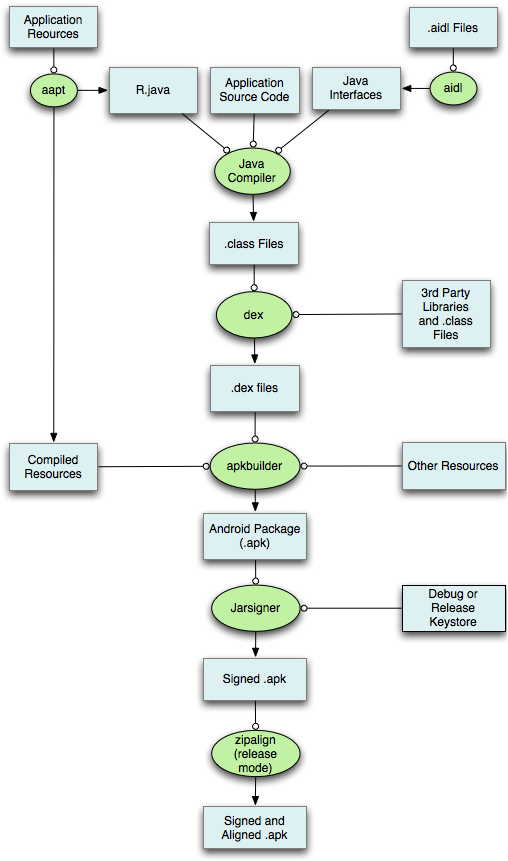
\includegraphics[scale=0.7]{fig/build.png}
    \caption{Build process}
    \label{buildProcess}
\end{figure}



